\section*{Appendix}
\label{sec:appendix}
\addcontentsline{toc}{section}{Appendix}
\appendix
\addtocontents{toc}{\protect\setcounter{tocdepth}{2}}
\makeatletter
\addtocontents{toc}{%
  \begingroup
  \let\protect\l@chapter\protect\l@section
  \let\protect\l@section\protect\l@subsection
}

\section{Benchmark Definitions}
\paragraph{Boundaries with filter} \mbox{}
\begin{lstlisting}[language=json,firstnumber=1]
{
  "name": "Join Time - Boundaries (Filter)",
  "benchmarks": [
    {
      "name": "Raven",
      "iterations": 5,
      "group": ["GLC", "SWF", "Treecover"],
      "command": {
        "path": "java",
        "args": [
          "-jar",
          "-Xmx14g",
          "/home/runners/raven-runner-1.0.jar",
          "-iv",
          "/home/real/vector/boundaries/ne_10m_admin_0_countries.shp",
          "-cl",
          "/home/raster-cache/",
          "-ir",
          [
            "/home/real/raster/glc2000",
            "/home/real/raster/woody",
            "/home/real/raster/treecover"
          ],
          "-t",
          "parallel",
          "-ts",
          "2048",
          "-fl",
          ["22", "1", "81"],
          "-fh",
          ["22", "1", "84"]
        ]
      },
      "environment_options": {
        "environment_type": "docker",
        "docker_file_path": "./runners/raven-runner/",
        "docker_mount_path": "/home/joinpro/data"
      }
    },
    {
      "name": "Raptor",
      "iterations": 5,
      "group": ["GLC", "SWF", "Treecover"],
      "command": {
        "path": "java",
        "args": [
          "-jar",
          "-Xmx14g",
          "/home/runners/raptor-runner-1.0.jar",
          "-iv",
          "/home/real/vector/boundaries/ne_10m_admin_0_countries.shp",
          "-ir",
          [
            "/home/real/raster/glc2000",
            "/home/real/raster/woody",
            "/home/real/raster/treecover"
          ],
          "-fl",
          ["22", "1", "81"],
          "-fh",
          ["22", "1", "84"]
        ]
      },
      "environment_options": {
        "environment_type": "docker",
        "docker_file_path": "./runners/raptor-runner/",
        "docker_mount_path": "/home/joinpro/data"
      }
    }
  ],
  "colours": {
    "Raven": "darkred",
    "Raptor": "darkblue"
  }
}
\end{lstlisting}

\newpage
\paragraph{Boundaries without filter} \mbox{}
\begin{lstlisting}[language=json,firstnumber=1]
{
  "name": "Join Time - Boundaries (No Filter)",
  "benchmarks": [
    {
      "name": "Raven",
      "iterations": 5,
      "group": ["GLC", "SWF", "Treecover"],
      "command": {
        "path": "java",
        "args": [
          "-jar",
          "-Xmx14g",
          "/home/runners/raven-runner-1.0.jar",
          "-iv",
          "/home/real/vector/boundaries/ne_10m_admin_0_countries.shp",
          "-cl",
          "/home/raster-cache/",
          "-ir",
          [
            "/home/real/raster/glc2000",
            "/home/real/raster/woody",
            "/home/real/raster/treecover"
          ],
          "-t",
          "parallel",
          "-ts",
          "2048"
        ]
      },
      "environment_options": {
        "environment_type": "docker",
        "docker_file_path": "./runners/raven-runner/",
        "docker_mount_path": "/home/joinpro/data"
      }
    },
    {
      "name": "Raptor",
      "iterations": 5,
      "group": ["GLC", "SWF", "Treecover"],
      "command": {
        "path": "java",
        "args": [
          "-jar",
          "-Xmx14g",
          "/home/runners/raptor-runner-1.0.jar",
          "-iv",
          "/home/real/vector/boundaries/ne_10m_admin_0_countries.shp",
          "-ir",
          [
            "/home/real/raster/glc2000",
            "/home/real/raster/woody",
            "/home/real/raster/treecover"
          ]
        ]
      },
      "environment_options": {
        "environment_type": "docker",
        "docker_file_path": "./runners/raptor-runner/",
        "docker_mount_path": "/home/joinpro/data"
      }
    }
  ],
  "colours": {
    "Raven": "darkred",
    "Raptor": "darkblue"
  }
}
\end{lstlisting}

\newpage
\paragraph{Protected Areas with filter} \mbox{}
\begin{lstlisting}[language=json,firstnumber=1]
{
  "name": "Join Time - Protected Areas (Filter)",
  "benchmarks": [
    {
      "name": "Raven",
      "iterations": 5,
      "group": ["GLC", "SWF", "Treecover"],
      "command": {
        "path": "java",
        "args": [
          "-jar",
          "-Xmx14g",
          "/home/runners/raven-runner-1.0.jar",
          "-iv",
          "/home/real/vector/protected_areas/ProtectedArea.shp",
          "-cl",
          "/home/raster-cache/",
          "-ir",
          [
            "/home/real/raster/glc2000",
            "/home/real/raster/woody",
            "/home/real/raster/treecover"
          ],
          "-fl",
          ["22", "1", "81"],
          "-fh",
          ["22", "1", "84"],
          "-t",
          "parallel",
          "-ts",
          "2048"
        ]
      },
      "environment_options": {
        "environment_type": "docker",
        "docker_file_path": "./runners/raven-runner/",
        "docker_mount_path": "/home/joinpro/data"
      }
    },
    {
      "name": "Raptor",
      "iterations": 5,
      "group": ["GLC", "SWF", "Treecover"],
      "command": {
        "path": "java",
        "args": [
          "-jar",
          "-Xmx14g",
          "/home/runners/raptor-runner-1.0.jar",
          "-iv",
          "/home/real/vector/protected_areas/ProtectedArea.shp",
          "-ir",
          [
            "/home/real/raster/glc2000",
            "/home/real/raster/woody",
            "/home/real/raster/treecover"
          ],
          "-fl",
          ["22", "1", "81"],
          "-fh",
          ["22", "1", "84"]
        ]
      },
      "environment_options": {
        "environment_type": "docker",
        "docker_file_path": "./runners/raptor-runner/",
        "docker_mount_path": "/home/joinpro/data"
      }
    }
  ],
  "colours": {
    "Raven": "darkred",
    "Raptor": "darkblue"
  }
}
\end{lstlisting}

\newpage
\paragraph{Protected Areas without filter} \mbox{}
\begin{lstlisting}[language=json,firstnumber=1]
{
  "name": "Join Time - Protected Areas (No Filter)",
  "benchmarks": [
    {
      "name": "Raven",
      "iterations": 5,
      "group": ["GLC", "SWF", "Treecover"],
      "command": {
        "path": "java",
        "args": [
          "-jar",
          "-Xmx14g",
          "/home/runners/raven-runner-1.0.jar",
          "-iv",
          "/home/real/vector/protected_areas/ProtectedArea.shp",
          "-cl",
          "/home/raster-cache/",
          "-ir",
          [
            "/home/real/raster/glc2000",
            "/home/real/raster/woody",
            "/home/real/raster/treecover"
          ],
          "-t",
          "parallel",
          "-ts",
          "2048"
        ]
      },
      "environment_options": {
        "environment_type": "docker",
        "docker_file_path": "./runners/raven-runner/",
        "docker_mount_path": "/home/joinpro/data"
      }
    },
    {
      "name": "Raptor",
      "iterations": 5,
      "group": ["GLC", "SWF", "Treecover"],
      "command": {
        "path": "java",
        "args": [
          "-jar",
          "-Xmx14g",
          "/home/runners/raptor-runner-1.0.jar",
          "-iv",
          "/home/real/vector/protected_areas/ProtectedArea.shp",
          "-ir",
          [
            "/home/real/raster/glc2000",
            "/home/real/raster/woody",
            "/home/real/raster/treecover"
          ]
        ]
      },
      "environment_options": {
        "environment_type": "docker",
        "docker_file_path": "./runners/raptor-runner/",
        "docker_mount_path": "/home/joinpro/data"
      }
    }
  ],
  "colours": {
    "Raven": "darkred",
    "Raptor": "darkblue"
  }
}
\end{lstlisting}

\newpage
\paragraph{Small Woody Features with filter} \mbox{}
\begin{lstlisting}[language=json,firstnumber=1]
{
  "name": "Join Time - Woody (Filter)",
  "benchmarks": [
    {
      "name": "Raven",
      "iterations": 5,
      "group": ["GLC", "SWF", "Treecover"],
      "command": {
        "path": "java",
        "args": [
          "-jar",
          "-Xmx14g",
          "/home/runners/raven-runner-1.0.jar",
          "-iv",
          "/home/real/vector/woody/woody.shp",
          "-cl",
          "/home/raster-cache/",
          "-ir",
          [
            "/home/real/raster/glc2000",
            "/home/real/raster/woody",
            "/home/real/raster/treecover"
          ],
          "-t",
          "parallel",
          "-ts",
          "2048",
          "-fl",
          ["22", "1", "81"],
          "-fh",
          ["22", "1", "84"]
        ]
      },
      "environment_options": {
        "environment_type": "docker",
        "docker_file_path": "./runners/raven-runner/",
        "docker_mount_path": "/home/joinpro/data"
      }
    },
    {
      "name": "Raptor",
      "iterations": 5,
      "group": ["GLC", "SWF", "Treecover"],
      "command": {
        "path": "java",
        "args": [
          "-jar",
          "-Xmx14g",
          "/home/runners/raptor-runner-1.0.jar",
          "-iv",
          "/home/real/vector/woody/woody.shp",
          "-ir",
          [
            "/home/real/raster/glc2000",
            "/home/real/raster/woody",
            "/home/real/raster/treecover"
          ],
          "-fl",
          ["22", "1", "81"],
          "-fh",
          ["22", "1", "84"]
        ]
      },
      "environment_options": {
        "environment_type": "docker",
        "docker_file_path": "./runners/raptor-runner/",
        "docker_mount_path": "/home/joinpro/data"
      }
    }
  ],
  "colours": {
    "Raven": "darkred",
    "Raptor": "darkblue"
  }
}
\end{lstlisting}

\newpage
\paragraph{Small Woody Features without filter} \mbox{}
\begin{lstlisting}[language=json,firstnumber=1]
{
  "name": "Join Time - Woody (No Filter)",
  "benchmarks": [
    {
      "name": "Raven",
      "iterations": 5,
      "group": ["GLC", "SWF", "Treecover"],
      "command": {
        "path": "java",
        "args": [
          "-jar",
          "-Xmx14g",
          "/home/runners/raven-runner-1.0.jar",
          "-iv",
          "/home/real/vector/woody/woody.shp",
          "-cl",
          "/home/raster-cache/",
          "-ir",
          [
            "/home/real/raster/glc2000",
            "/home/real/raster/woody",
            "/home/real/raster/treecover"
          ],
          "-t",
          "parallel",
          "-ts",
          "2048"
        ]
      },
      "environment_options": {
        "environment_type": "docker",
        "docker_file_path": "./runners/raven-runner/",
        "docker_mount_path": "/home/joinpro/data"
      }
    },
    {
      "name": "Raptor",
      "iterations": 5,
      "group": ["GLC", "SWF", "Treecover"],
      "command": {
        "path": "java",
        "args": [
          "-jar",
          "-Xmx14g",
          "/home/runners/raptor-runner-1.0.jar",
          "-iv",
          "/home/real/vector/woody/woody.shp",
          "-ir",
          [
            "/home/real/raster/glc2000",
            "/home/real/raster/woody",
            "/home/real/raster/treecover"
          ]
        ]
      },
      "environment_options": {
        "environment_type": "docker",
        "docker_file_path": "./runners/raptor-runner/",
        "docker_mount_path": "/home/joinpro/data"
      }
    }
  ],
  "colours": {
    "Raven": "darkred",
    "Raptor": "darkblue"
  }
}
\end{lstlisting}

\newpage
\paragraph{Cache Build Time} \mbox{}
\begin{lstlisting}[language=json,firstnumber=1]
{
  "name": "Cache Build Time",
  "benchmarks": [
    {
      "name": "Raven",
      "iterations": 3,
      "group": [
        "GLC2000",
        "SWF",
        "Treecover"
      ],
      "command": {
        "path": "java",
        "args": [
          "-jar",
          "-Xmx14g",
          "/home/runners/raven-runner-1.0-BUILD-TIME.jar",
          "-iv",
          "/home/real/vector/boundaries/ne_10m_admin_0_countries.shp",
          "-cl",
          "/home/build-raster-cache/",
          "-ir",
          [
            "/home/real/raster/glc2000",
            "/home/real/raster/woody",
            "/home/real/raster/treecover"
          ],
          "-t",
          "parallel",
          "-c",
          "false",
          "-ts",
          "2048"
        ]
      },
      "environment_options": {
        "environment_type": "docker",
        "docker_file_path": "./runners/raven-runner/",
        "docker_mount_path": "/home/joinpro/data"
      }
    }
  ],
  "colours": {
    "Raven": "darkred",
    "Raptor": "darkblue"
  }
}
\end{lstlisting}



\section{Inner \rtree Type}
\label{sec:inner-r-tree}

\begin{figure}[H]
    \centering
    \includegraphics[width=\textwidth]{images/08appendix/R-tree Type (GLC2000) .png}
    \caption{}
    \label{fig:rtree-extra1}
\end{figure}
\begin{figure}[H]
    \centering
    \includegraphics[width=\textwidth]{images/08appendix/R-tree Type (GLC2000) (No Filter) .png}
    \caption{}
    \label{fig:rtree-extra2}
\end{figure}
\begin{figure}[H]
    \centering
    \includegraphics[width=\textwidth]{images/08appendix/R-tree Type (Treecover) .png}
    \caption{ }
    \label{fig:rtree-extra3}
\end{figure}

\label{app:bench}


\section{\rtree Load Comparison with Real Data}
\label{app:r-tree-comparison}
For each of the groups in figure \ref{fig:r*-tree-all} and figure \ref{fig:str-tree-all}, the raster sets are in the following order: \textit{GLC2000}, \textit{Treecover} and \textit{Small Woody Features (raster)}.
\begin{figure}[H]
    \centering
    \includegraphics[width=\textwidth]{images/08appendix/Join Time - All (R-star) .png}
    \caption{Join time for all datasets using a \rstar}
    \label{fig:r*-tree-all}
\end{figure}

\begin{figure}[H]
    \centering
    \includegraphics[width=\textwidth]{images/08appendix/Join Time - All (STR) .png}
    \caption{Join time for all datasets using a \str}
    \label{fig:str-tree-all}
\end{figure}

\section{Datasets}

\subsection{Vector}

\subsubsection{Boundaries}
\begin{figure}[H]
    \centering
    \includegraphics[width=\textwidth]{images/08appendix/boundaries.png}
    \caption{The entire \textit{Boundaries} dataset.}
    \label{fig:boundaries-example}
\end{figure}
\subsubsection{Protected Areas}
\begin{figure}[H]
    \centering
    \includegraphics[width=\textwidth]{images/08appendix/protected.png}
    \caption{The entire \textit{Protected Areas} dataset.}
    \label{fig:protected-areas-example}
\end{figure}
\subsubsection{Small Woody Features}
\begin{figure}[H]
    \centering
    \includegraphics[width=\textwidth]{images/08appendix/SWF.png}
    \caption{The entire \textit{SWF (vector)} dataset in black.}
    \label{fig:SWF-vector-example-2}
\end{figure}

\begin{figure}[H]
    \centering
    \includegraphics[width=\textwidth]{images/08appendix/SWF_DETAILED.png}
    \caption{A snippet of \textit{SWF (vector)}.}
    \label{fig:SWF-vector-example-1}
\end{figure}



\subsection{Raster}

\subsubsection{GLC2000}
\begin{figure}[H]
    \centering
    \includegraphics[width=\textwidth]{images/08appendix/glc-example.png}
    \caption{Crop of \textit{GLC2000}.}
    \label{fig:glc2000-example}
\end{figure}

\subsubsection{Treecover}
\begin{figure}[H]
    \centering
    \includegraphics[width=\textwidth]{images/08appendix/treecover-example.png}
    \caption{Example of a \textit{Treecover} tile imported to Google Earth.}
    \label{fig:treecover-example}
\end{figure}

\subsubsection{Small Woody Features}

\begin{figure}[H]
    \centering
    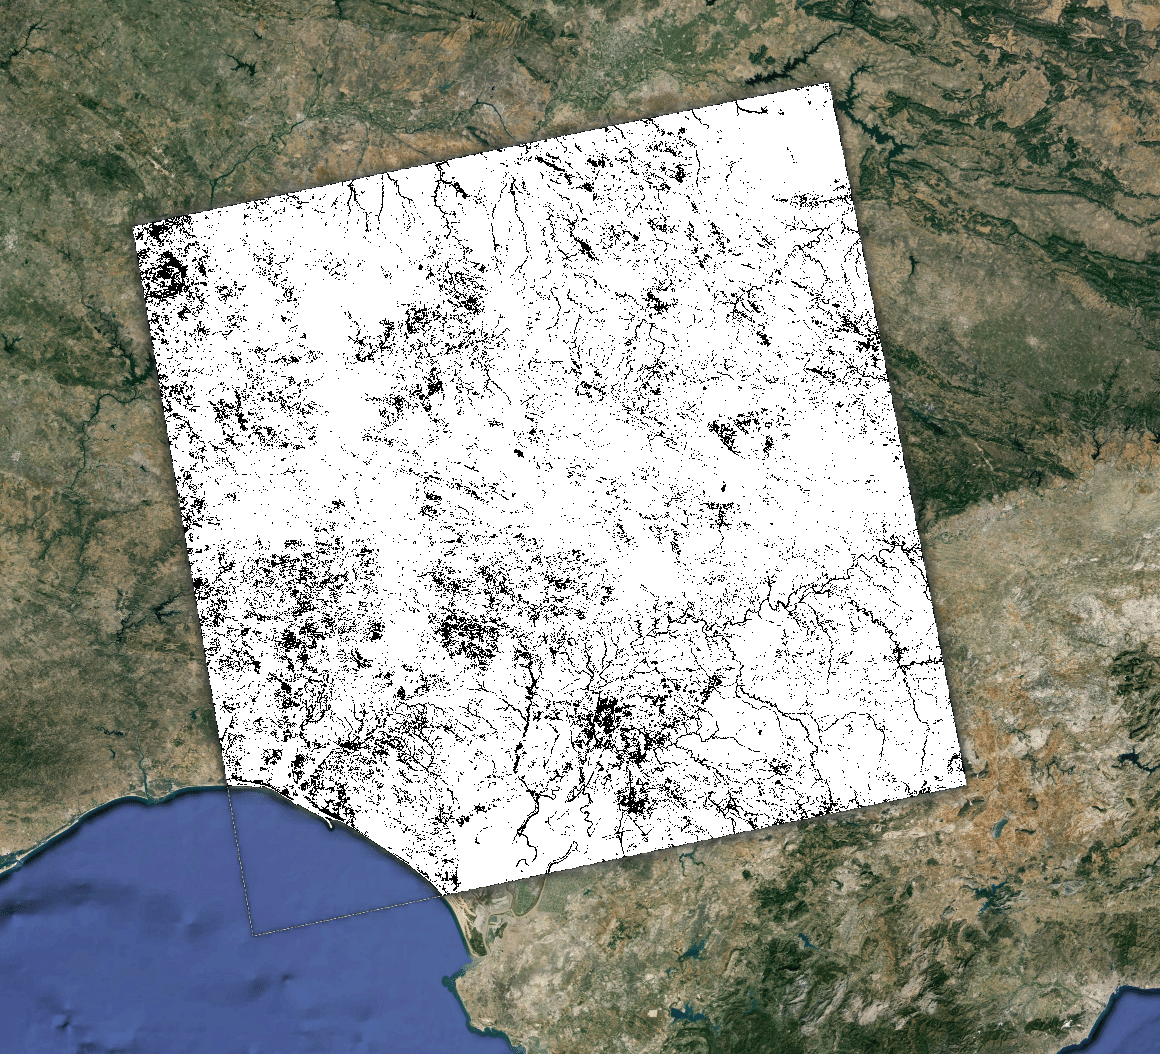
\includegraphics[width=\textwidth]{images/08appendix/swf-raster-example.png}
    \caption{Example of a \textit{Small Woody Features (raster)} tile imported to Google Earth. Visually enhanced by being converted to black and white.}
    \label{fig:SWF-raster-example}
\end{figure}